\documentclass[12pt, letterpaper]{article}
\usepackage[margin=1.0in]{geometry}
\usepackage{graphicx}
\usepackage{listings}

\begin{document}
\title{Predicting Boston Housing Prices}
\author{Nubyra Ahmed}
\maketitle 

\section{Statistical Analysis and Data Exploration}

Below is a descriptive summary of the dataset, including a box plot displaying data distribution.\\

\begin{center}
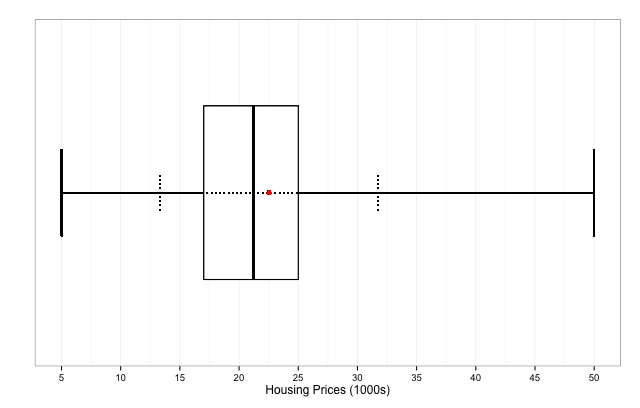
\includegraphics[width=13cm,height=7cm]{boxplot}
\end{center}

\begin{itemize}
\item Sample Size: 506
\item Number of Features: 13
\item Minimum Housing Price: 5.0
\item Maximum Housing Price: 50.0
\item Mean Housing Price: 22.5
\item Median Housing Price: 21.2
\item Standard Deviation of Housing Prices: 9.2
\end{itemize}

\section{Evaluating Model Performance}

Predicting Boston housing prices is a regression problem, since the response variable (housing prices) is continuous. Therefore, when evaluating model performance we need to consider performance metrics for regression. 

\subsection{Measure of Model Performance}

Two metrics are considered as candidates for measuring model performance, the Mean Absolute Error (MAE) and the Mean Squared Error (MSE). MAE and MSE is calculated using Equation \ref{mae} and \ref{mse}, respectively,  where $y_i$ is the true response value and $\hat y_i$ is the predicted value for the $i^{th}$ sample. 

 \begin{equation}
 \label{mae}
    MAE = \frac{1}{n}\sum_{i=1}^{n}|y_i-\hat y_i|
 \end{equation}
 
 \begin{equation}
 \label{mse}
    MSE = \frac{1}{n}\sum_{i=1}^{n}(y_i-\hat y_i)^2
 \end{equation}
 
The goal of both metrics is to determine the average relative distance of the predicted from the true value, while ensuring that negative differences do not cancel out positive differences. In MAE this is achieved by taking the absolute value of the differences. While in MSE the difference is squared. 

There are several attractive benefits to using MSE. It is a differentiable function, as a result allows us to find the minimum or maximum values. By taking the square of the errors, the larger errors are emphasized, rather than the smaller ones. For instance an absolute error of $.1$ will account for $.01$ in the summation, versus an error of $10$ will account for $100$. Therefore, MSE was chosen as the performance metric for this regression problem. 

\subsection{Importance of Splitting the Data}

In an ideal word we would have access to unlimited data points, in such case we would choose the model that has the lowest error rate on the entire population, as a result the error rate is the true error rate. However, in the real world we have access to finite number of data points. In such case if we used the entire dataset to determine the final model, the final model will likely overfit the training data and error rate will be optimistic. A solution to this problem is to split the data into training and testing set, called the holdout method. The training set is used to build the learning algorithm, and the test set is used to estimate the error rate of the trained model to determine how well our model would predict in the real world. 

\subsection{Cross Validation}

There are several disadvantages to splitting the data and applying the holdout method. Ideally we would want to maximize the number of data points in both training and testing set for selecting the best performing model. Also, since we randomly split the data only once, the estimated error rate will be misleading if we happen to get an ``unfortunate" split. An alternative approach to overcoming these disadvantages is Cross Validation (CV). There are three major CV techniques. 

\begin{enumerate}
\item In random subsampling, $K$ data splits are performed. In each split, a fixed number of data points are randomly selected without replacement as the test set. For each split, model is trained and estimated error rate is obtained. The true error estimate is the average the K error estimates.
\item In $K$-Fold CV, data is split into $K$ subsets, and the holdout method is repeated $K$ times. Each time one of the $K$ subsets is used as the test set and the remaining $K$-1 subsets are used as the training set. Then the average true error estimate is based on the $K$ models. An advantage of $K$-Fold CV is that all the data points are eventually used in the training and testing set.  
\item In Leave-one-out, for $n$ sample size, build n models, using $n$-1 data points for training and the remaining example for testing. Then the average true error estimate is based on the $n$ models.
\end{enumerate}

\subsection{Grid Search}

Learning algorithms have parameters or typically called hyper parameters that are not automatically learned by the model. These hyperparameters need to tuned for optimal performance. An optimal way of tuning these parameters is via grid search method, where one has to specify a set of possible values for the hyperparameters(s) and train a model for each of the combination of parameter values lying in a grid and evaluate the models using cross-validation. Final model is the the one that had the best performance. 

\section{Analyzing Model Performance}

For predicting Boston housing prices, MSE was chosen as the performance metric and Decision Tree Regression was chosen as the learning algorithm to be optimized. Grid search with Cross Validation approach was applied to find the optimal maximum depth for the decision tree, where the default $K$-Fold CV was used for validating model performance. 

\subsection{General Trend}

To evaluate Decision Tree performance, 10 graphs were plotted for each level of maximum depth 1 to 10. As the tree depths increased, training error decreased with sample size, by maximum depth of 10, training error was near zero. For testing error, from maximum depth of 4 to 6, error rate seems to decrease and remain around the same and then starts increasing as maximum depth increases. 

\subsection{Bias and Variance}

From the learning curve shown below for model performance at maximum depth of 1, it is clear that this model suffers from high bias. Due to lack of model complexity, the model is unable to learn the relationship between the features and housing prices.

\begin{center}
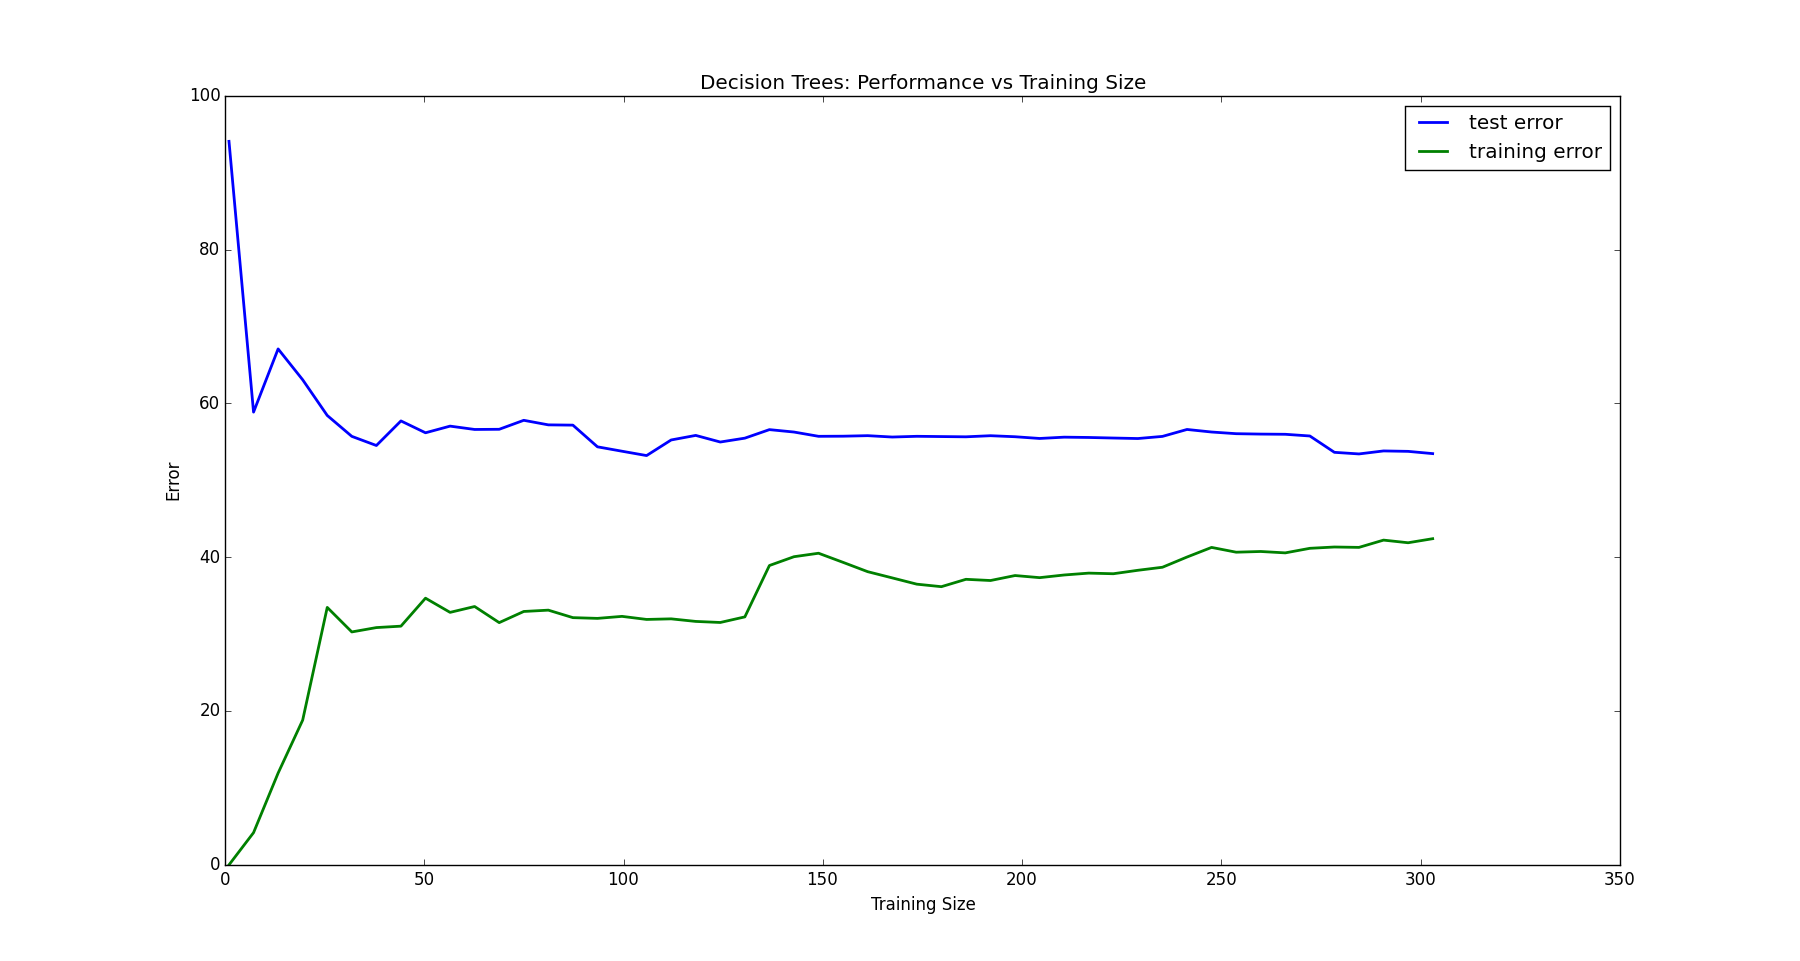
\includegraphics[width=13cm,height=8cm]{DT1}
\end{center}

On the other hand, learning curve shown below for model performance at maximum depth of 10, the model seems to overfit, leading to high variance. The training error is near zero and testing error seems to be higher than previous models.

\begin{center}
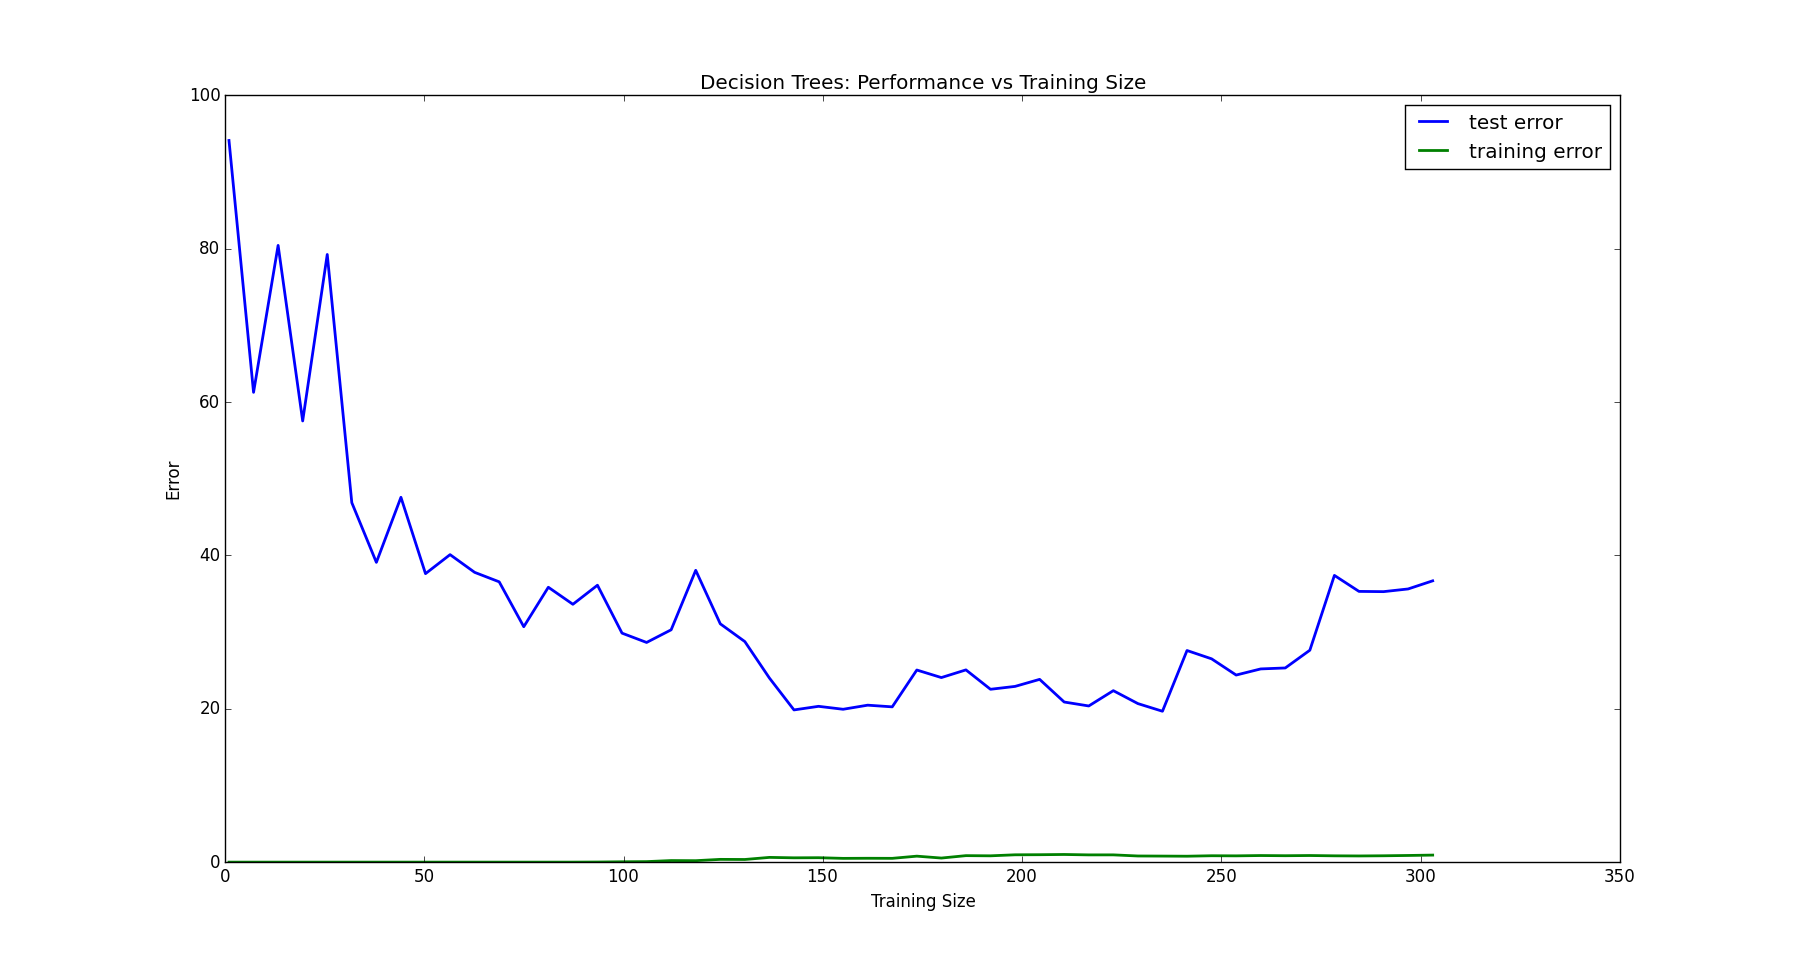
\includegraphics[width=13cm,height=8cm]{DT10}
\end{center}

\newpage

\subsection{Model Complexity}

\begin{center}
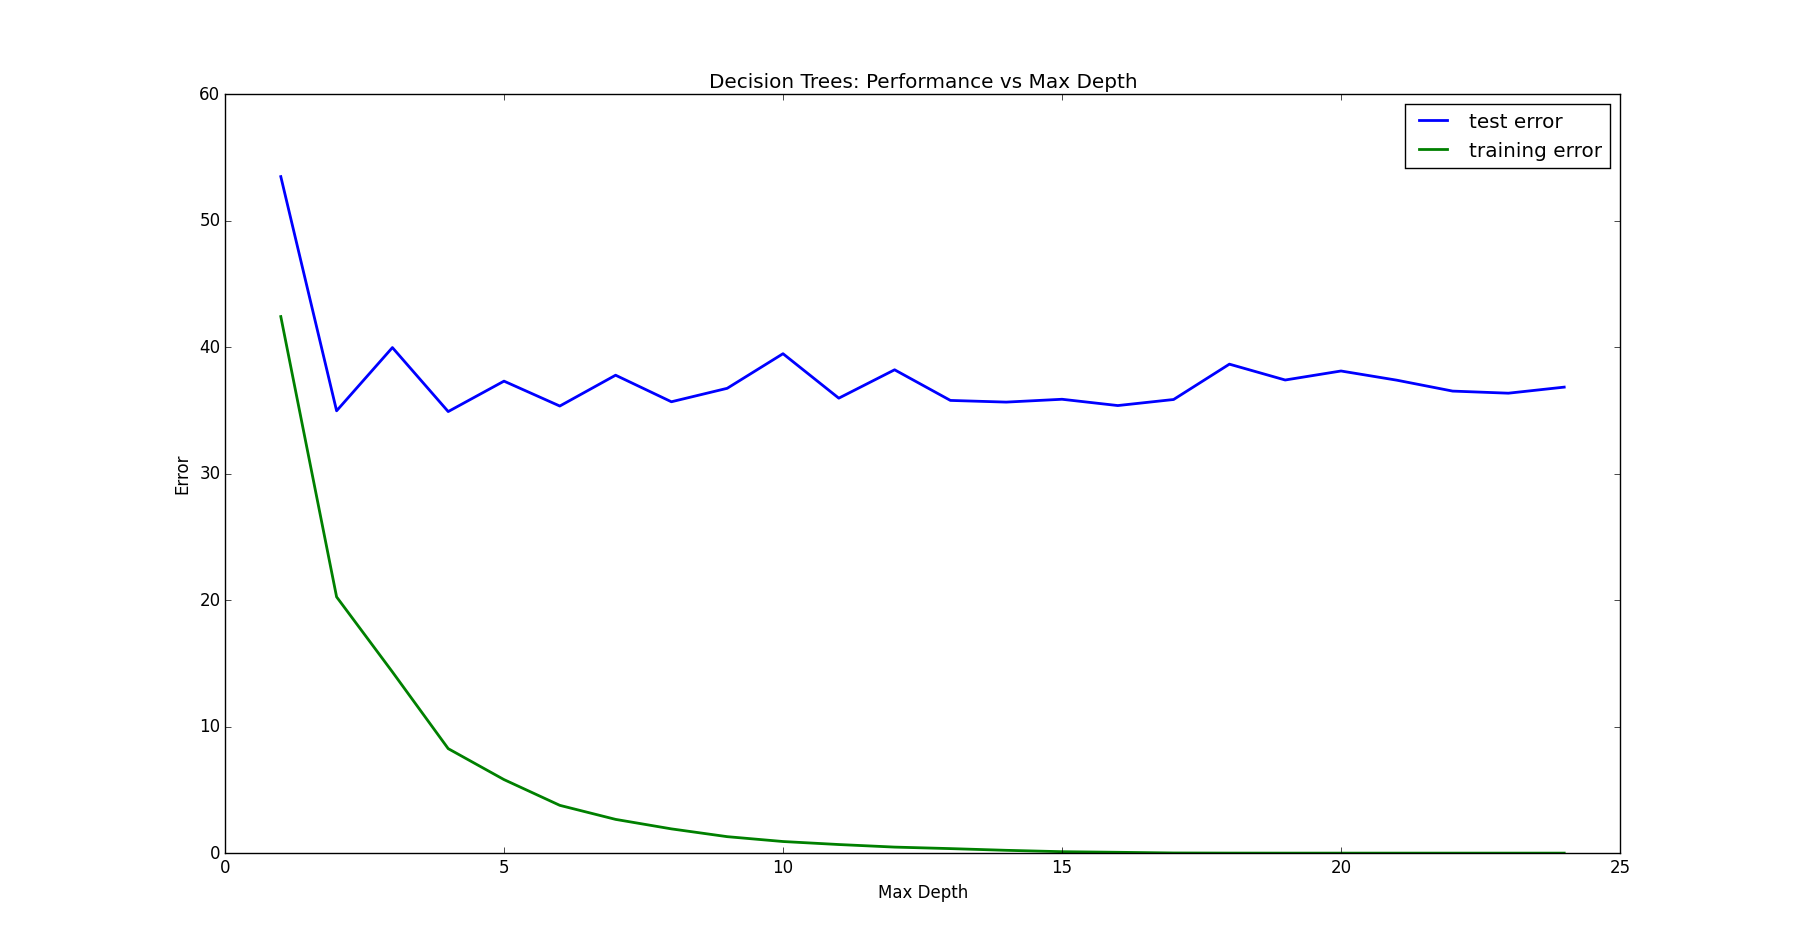
\includegraphics[width=13cm,height=8cm]{Model}
\end{center}

As suggested by the model complexity graph above, as maximum depth increases, training error decreases, eventually starting to plateau toward zero after maximum depth of of around 4 or 5. Due to the small randomization, the grid search with CV method was run 10 times, 8 out of 10 times, the best maximum depth obtained was 4. This suggests that optimal decision tree is obtained using maximum depth of 4. Below is an output of grid search with best max depth of 4. 

\begin{lstlisting}
DecisionTreeRegressor(criterion='mse', max_depth=4, max_features=None,
max_leaf_nodes=None, min_samples_leaf=1, min_samples_split=2,
min_weight_fraction_leaf=0.0, random_state=None, splitter='best')
\end{lstlisting}

\section{Model Prediction}

A decision tree with maximum depth of 4 is our final model. Below is an example of a house with the listed feature values and its prediction.\\\\
House: [11.95, 0.0, 18.1, 0, 0.659, 5.609, 90.0, 1.385, 24, 680.0, 20.2, 332.09, 12.13]\\
Prediction: [ 21.62974359]\\\\
The predicted housing price is within one standard deviation of the mean housing prices, and it is about the same value as the median housing prices.


\end{document}